
\section{Gated Van-der-Pauw Method}

\begin{figure}[htbp]
\centering
\resizebox{0.8\textwidth}{!}{\input{figures/tikz/circuit-gvdP.tex}}
\caption[Gated van der Pauw measurement circuit]{Gated van der Pauw measurement circuit used to extract the intrinsic sheet conductance. A constant current $I_\text{34}$ is driven between contacts 3 and 4 while the voltage $V_\text{34}$ is monitored. The transverse probe voltages $V_\text{14}$ and $V_\text{24}$ are measured with high-impedance voltmeters, and the gate branch applies $V_\text{G4}$ while monitoring the leakage current $I_\text{G4}$. Adapted from Ref.~\cite{Kersting2026FiguresCollection}.}
\label{fig:gated_vdp_circuit}
\end{figure}




\subsection{Extraction of Intrinsic Mobility and Threshold Voltage}

The gated van der Pauw measurement was used to separate the intrinsic sheet transport of the accumulated semiconductor film from the contact resistance of the injecting electrodes~\cite{Rolin2017GVDP,Lee2024GVDPIGZO}. A constant current $I_{34}$ is driven through the device, while the voltage probes measure the transverse van der Pauw voltage with negligible current draw. From the measured sheet conductance $\sigma$, the intrinsic mobility and threshold voltage are obtained from the linear gate-voltage dependence of the conductance,
\begin{equation}
\sigma = \mu C_\mathrm{i}\left(V_\mathrm{eff}-V_\mathrm{T,eff}\right),
\qquad
\mu=\frac{1}{C_\mathrm{i}}\frac{\mathrm{d}\sigma}{\mathrm{d}V_\mathrm{eff}},
\qquad
V_\mathrm{eff}=-(V_\text{G4}-V_\text{C}),
\end{equation}
where $C_\mathrm{i}=\SI{2}{\nano\farad}/\SI{32}{\milli\metre\squared}=\SI{6.25}{\nano\farad\per\centi\metre\squared}$ is the gate-insulator capacitance per unit area. The slope of the conductance fit gives the intrinsic mobility, while the extrapolated intercept gives the threshold voltage. 

\begin{figure}[htbp]
\centering
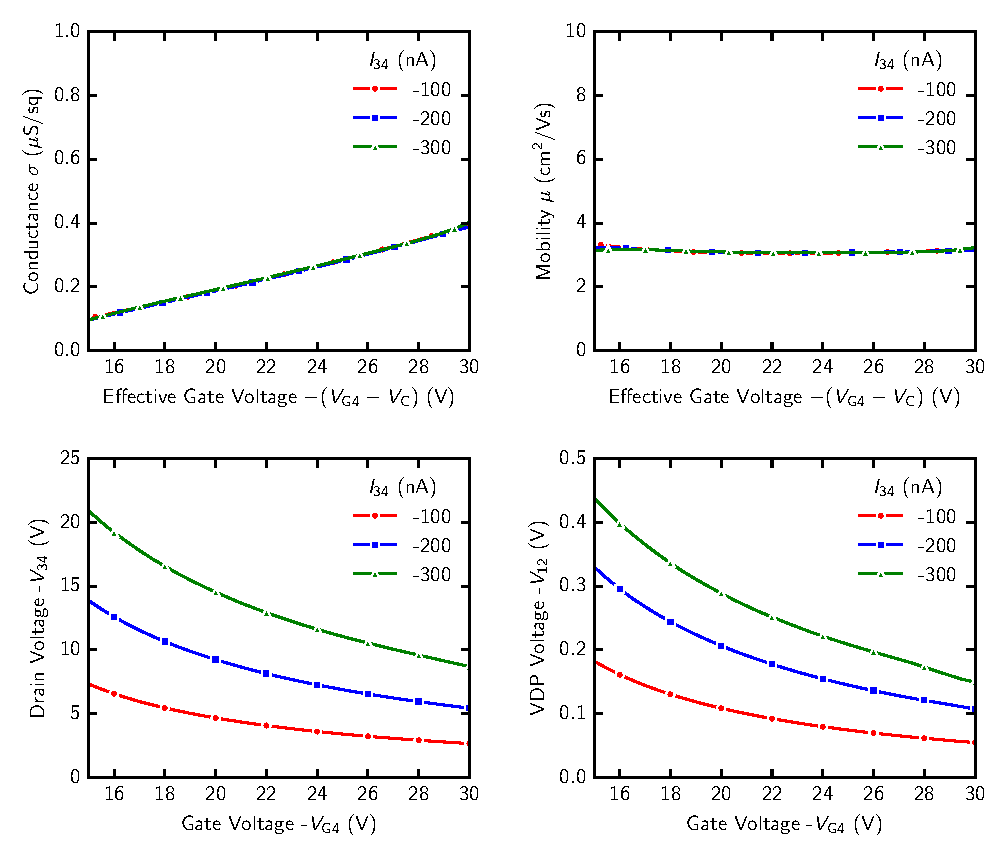
\includegraphics[width=\textwidth]{figures/gvdP}
\caption[Gated van der Pauw extraction of intrinsic sheet conductance, mobility, and threshold voltage]{Gated van der Pauw extraction of the intrinsic sheet conductance, mobility, and threshold voltage for three applied currents, $I_{34}=\SI{-100}{\nano\ampere}$, $\SI{-200}{\nano\ampere}$, and $\SI{-300}{\nano\ampere}$. The bottom panels show the measured drain voltage $-V_{34}$ and van der Pauw voltage $-V_{12}$ as functions of gate voltage. Both voltages decrease as the negative gate bias increases, because the accumulated channel becomes more conductive. The top-left panel shows the resulting sheet conductance $\sigma$ as a function of effective gate voltage $-(V_\text{G4}-V_\text{C})$, and the top-right panel shows the mobility extracted from the conductance slope. The collapse of the data for different currents indicates linear-response behaviour and supports a current-independent extraction of both mobility and threshold voltage.}
\label{fig:gated_vdp_intrinsic_mobility}
\end{figure}

Figure~\ref{fig:gated_vdp_intrinsic_mobility} summarizes the complete extraction procedure. In the raw voltage data, the magnitude of $-V_{34}$ increases with the applied current, as expected from Ohm's law, but it decreases with increasing $-V_\text{G4}$ because the gate bias creates a denser hole-accumulation layer. The van der Pauw voltage $-V_{12}$ follows the same trend and is smaller than the longitudinal voltage because it probes the lateral sheet resistance rather than the full source--drain voltage drop.

After conversion to sheet conductance, the three current series collapse onto a single nearly linear curve. This current independence is important because it shows that the sheet conductance is not an artefact of the chosen current bias or of self-heating~\cite{Rolin2017GVDP}. The linear increase of $\sigma$ with effective gate voltage indicates that the induced sheet charge is approximately proportional to the gate overdrive in this voltage range. The extracted mobility is nearly constant, showing that the gated van der Pauw method yields a stable intrinsic mobility in contrast to two-terminal measurements, where contact resistance and injection barriers can strongly distort the apparent mobility~\cite{Bittle2016MobilityOverestimation,Natali2012ChargeInjection}.

\begin{table}[htbp]
\centering
\begin{tabular}{|c|c|c|c|}
\hline
$I_{34}$ (nA) & $\mu$ (\si{cm^2/Vs}) & $V_\text{T}$ (V) & $R^2$ \\
\hline
$-100$ & $3.11 \pm 0.02$ & $-10.16 \pm 0.20$ & $0.9981$ \\
$-200$ & $3.11 \pm 0.02$ & $-10.31 \pm 0.16$ & $0.9987$ \\
$-300$ & $3.10 \pm 0.02$ & $-10.11 \pm 0.13$ & $0.9991$ \\
\hline
\end{tabular}
\caption[Fit results from gated van der Pauw conductance analysis]{Fit results from the linear conductance analysis in Figure~\ref{fig:gated_vdp_intrinsic_mobility}. The mobility is obtained from the conductance slope, and the threshold voltage is obtained from the extrapolated intercept.}
\label{tab:gated_vdp_fit_results}
\end{table}

The fit results are listed in Table~\ref{tab:gated_vdp_fit_results}. The mobility values agree within their uncertainties for all three applied currents, giving an intrinsic mobility of approximately \SI{3.1}{\centi\metre\squared\per\volt\per\second}. The threshold voltages are also consistent, with values clustered around \SI{-10.2}{\volt}. The high coefficients of determination, $R^2>0.998$, confirm that the conductance is well described by a linear dependence on effective gate voltage over the fitted range. The small variation of both $\mu$ and $V_\text{T}$ with current demonstrates that the extraction is robust and that the gated van der Pauw geometry successfully suppresses contact-related artefacts in the mobility and threshold-voltage analysis. 


% \subsection{Temperature Analysis of Intrinsic Mobility}

% The intrinsic mobility extracted with the gated van der Pauw method was measured as a function of temperature to identify the dominant transport mechanism in the organic semiconductor. Temperature-dependent measurements are particularly useful for organic thin films because charge transport is often thermally activated. At lower temperature, carriers have less thermal energy to escape localized states or overcome energetic disorder, so the mobility is expected to decrease if hopping or trap-limited transport dominates.

% \begin{figure}[htbp]
% \centering
% \resizebox{0.75\textwidth}{!}{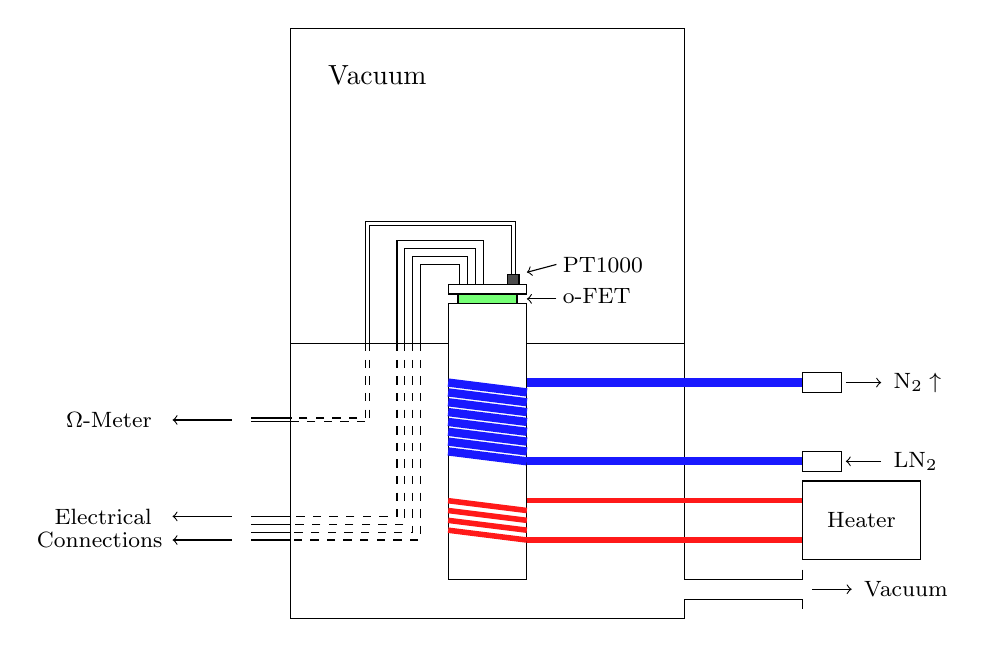
\begin{tikzpicture}[scale=0.5]

\draw [] (-1,2)--(-5,2)--(-5,-5)--(5,-5)--(5,-4.5)--(8,-4.5)--++(0,-0.25);

\draw [] (8,-3.75)--(8,-4)--(5,-4)--(5,2)--(1,2);
\draw[->] (8.25,-4.25)--++(1,0) node[right=1pt]{\footnotesize{Vacuum}};
% Solenoid core
\draw [] (-1,3)--(-1,-4)--(1,-4)--(1,3)--(-1,3);


\draw[] (8,-1.25)--(8,-0.75)--(9,-0.75)--(9,-1.25)--(8,-1.25);

\draw[] (8,1.25)--(8,0.75)--(9,.75)--(9,1.25)--(8,1.25);

\draw[->] (10,-1)--(9.1,-1);
\draw[->] (9.1,1)--(10,1);

\node at(10,1) [right=1pt]{\footnotesize{N$_2\uparrow$}};
\node at(10,-1) [right=1pt]{\footnotesize{LN$_2$}};


\draw[blue!90, line width = 3pt] (1,1)--(8,1);
\draw[blue!90, line width = 3pt] (1,-1)--(8,-1);
\draw[blue!90, line width = 3pt] (-1,1)--(1,0.75);
\draw[blue!90, line width = 3pt] (-1,0.75)--(1,0.5);
\draw[blue!90, line width = 3pt] (-1,0.5)--(1,0.25);
\draw[blue!90, line width = 3pt] (-1,0.25)--(1,0);
\draw[blue!90, line width = 3pt] (-1,0.0)--(1,-0.25);
\draw[blue!90, line width = 3pt] (-1,-0.25)--(1,-0.5);
\draw[blue!90, line width = 3pt] (-1,-0.5)--(1,-0.75);
\draw[blue!90, line width = 3pt] (-1,-0.75)--(1,-1);

\draw[red!90, line width = 2pt] (1,-2)--(8,-2);
\draw[red!90, line width = 2pt] (1,-3)--(8,-3);
\draw[red!90, line width = 2pt] (-1,-2)--(1,-2.25);
\draw[red!90, line width = 2pt] (-1,-2.25)--(1,-2.5);
\draw[red!90, line width = 2pt] (-1,-2.5)--(1,-2.75);
\draw[red!90, line width = 2pt] (-1,-2.75)--(1,-3);

\draw[] (8,-1.5)--(8,-3.5)--(11,-3.5)--(11,-1.5)--(8,-1.5);
\node at (9.5,-2.5) []{\footnotesize{Heater}};

\draw [fill = green!90, fill opacity = 0.6] (-0.75,3)--(-0.75,3.25)--(0.75,3.25)--(0.75,3)--(-0.75,3);
\node at (0.75,3.2) [right = 13pt]{\footnotesize{o-FET}};
\draw[->] (1.75,3.125)--(1,3.125);

\draw[](-0.70,3.5)--++(0,0.5)--++(-1,0)--++(0,-2);
\draw[dashed](-1.7,2)--++(0,-5)--++(-3.3,0);
\draw[](-5,-3)--(-6,-3);

\draw[](-0.5,3.5)--++(0,0.7)--++(-1.4,0)--++(0,-2.2);
\draw[dashed](-1.9,2)--++(0,-5+0.2)--++(-3.3+0.2,0);
\draw[](-5,-3+0.2)--(-6,-3+0.2);


\draw[](-0.5+0.2,3.5)--++(0,0.7+0.2)--++(-1.8,0)--++(0,-2.2-0.2);
\draw[dashed](-1.9-0.2,2)--++(0,-5+0.2+0.2)--++(-3.3+0.2+0.2,0);
\draw[](-5,-3+0.4)--(-6,-3+0.4);

\draw[](-0.5+0.2+0.2,3.5)--++(0,0.7+0.2+0.2)--++(-2.2,0)--++(0,-2.2-0.2-0.2);
\draw[dashed](-1.9-0.2-0.2,2)--++(0,-5+0.2+0.2+0.2)--++(-3.3+0.2+0.2+0.2,0);
\draw[](-5,-3+0.6)--(-6,-3+0.6);

\draw[->] (-6.5, -2.4) --(-8,-2.4) node[left=4pt]{\footnotesize{Electrical}};
\draw[->] (-6.5, -3) --(-8,-3) node[left=0.1pt]{\footnotesize{Connections}};


\draw [] (-1,3.25)--(-1,3.5)--(1,3.5)--(1,3.25)--(-1,3.25);
\draw [fill = black!70] (0.5,3.5)--(0.5,3.75)--(0.8,3.75)--(0.8,3.5)--(0.5,3.5);
\draw[] (0.6,3.75)--(0.6,5)--(-3,5)--(-3,2);
\draw[dashed] (-3,2)--(-3,0)--(-5,0);
\draw[](-5,0)--++(-1,0);


\draw[] (0.7,3.75)--(0.7,5.1)--(-3.1,5.1)--(-3.1,2);
\draw[dashed] (-3.1,2)--(-3.1,0.1)--(-5,0.1);
\draw[](-5,0.1)--++(-1,0);
\draw[->] (-6.5, 0.05) --++(-1.5,0) node[left=4pt]{\footnotesize{$\Omega$-Meter}};


\draw [] (-5,2)--(-5,10)--(5,10)--(5,2);

\node at (-5,10) [below right = 10pt]{Vacuum};

\node at (0.75,4.0) [right = 13pt]{\footnotesize{PT1000}};
\draw[->] (1.75,4.0)--(1.0,3.8);

\end{tikzpicture}}
% \caption[Cryostat setup for temperature-dependent mobility measurements]{Cryostat setup used for temperature-dependent intrinsic-mobility measurements. The OFET is mounted in the vacuum chamber and contacted electrically from outside the cryostat. Liquid nitrogen provides cooling through the cold line, evaporated nitrogen leaves the system as gas, and the heater together with the PT1000 temperature sensor enables controlled temperature stabilization during the gated van der Pauw measurement.}
% \label{fig:cryostat_temperature_setup}
% \end{figure}

% The measurement setup is shown schematically in Figure~\ref{fig:cryostat_temperature_setup}. The sample is placed in vacuum to reduce water adsorption and avoid uncontrolled heat exchange with the surrounding atmosphere. Liquid nitrogen is used to cool the sample stage, while the heater allows the temperature to be set and stabilized at selected values. At each temperature, the gated van der Pauw measurement is repeated so that the sheet conductance and the corresponding intrinsic mobility can be extracted under comparable electrical conditions.

% For thermally activated transport, the mobility can be described by an Arrhenius relation,
% \[
% \mu(T)=\mu_0\exp\left(-\frac{E_\text{a}}{k_\text{B}T}\right),
% \]
% where $\mu_0$ is a prefactor, $E_\text{a}$ is the activation energy, $k_\text{B}$ is the Boltzmann constant, and $T$ is the absolute temperature. Therefore, plotting the mobility on a logarithmic scale as a function of inverse temperature gives a straight line when one thermally activated process dominates. The slope of this line is proportional to $-E_\text{a}/k_\text{B}$ and can be used to estimate the energetic barrier for charge transport.

% \begin{figure}[htbp]
% \centering
% 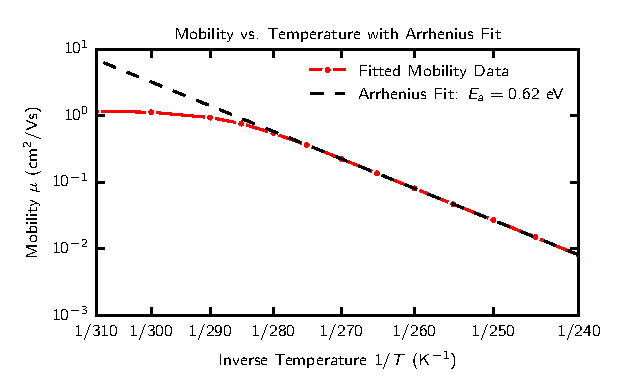
\includegraphics[scale=1]{figures/arrhenius}
% \caption[Arrhenius analysis of intrinsic mobility]{Arrhenius analysis of the intrinsic mobility extracted from the gated van der Pauw measurements. The mobility decreases strongly when the temperature is lowered from approximately \SI{310}{\kelvin} to \SI{240}{\kelvin}. The dashed line shows an Arrhenius fit to the thermally activated region, yielding an activation energy of $E_\text{a}=\SI{0.62}{\electronvolt}$.}
% \label{fig:arrhenius_intrinsic_mobility}
% \end{figure}

% Figure~\ref{fig:arrhenius_intrinsic_mobility} shows the extracted mobility as a function of inverse temperature. The mobility is highest near the highest measured temperature and decreases by roughly two orders of magnitude as the temperature is reduced. This strong temperature dependence confirms that the intrinsic transport is not band-like in this temperature range. Instead, it is consistent with thermally activated hopping or trap-limited transport through localized states in the organic semiconductor.

% The Arrhenius fit gives an activation energy of $E_\text{a}=\SI{0.62}{\electronvolt}$. This value represents the effective energy scale that carriers must overcome to contribute to long-range transport. It includes the influence of energetic disorder, trap states, and the temperature-dependent occupation of localized states. Small deviations from the fit at the highest temperatures indicate that the mobility does not follow a single activated process over the entire temperature range. Nevertheless, the approximately linear behaviour over most of the inverse-temperature range shows that thermal activation is the dominant trend. The temperature analysis therefore supports the interpretation that the mobility extracted by the gated van der Pauw method reflects intrinsic transport in a disordered organic semiconductor, rather than being limited only by contact resistance.